\documentclass[journal]{IEEEtran}
\usepackage{epsfig}
\usepackage[T1]{fontenc}
\usepackage[utf8]{vietnam}
\usepackage{enumerate}
\usepackage{amsmath}
\usepackage{amsfonts}
\usepackage{amssymb}
\usepackage{graphicx}
\usepackage{subfigure}
\usepackage{lmodern}
\setlength{\parskip}{0.5em}

\title{Test}
\author{HgN}

\begin{document}

\title{Tạo dựng khuôn mặt em bé}
\author{Hoang Gia Nguyen\\
Bach Khoa University, Vietnam\\}

\maketitle

\begin{center}
    \begin{figure}[!ht]
    \begin{center}
     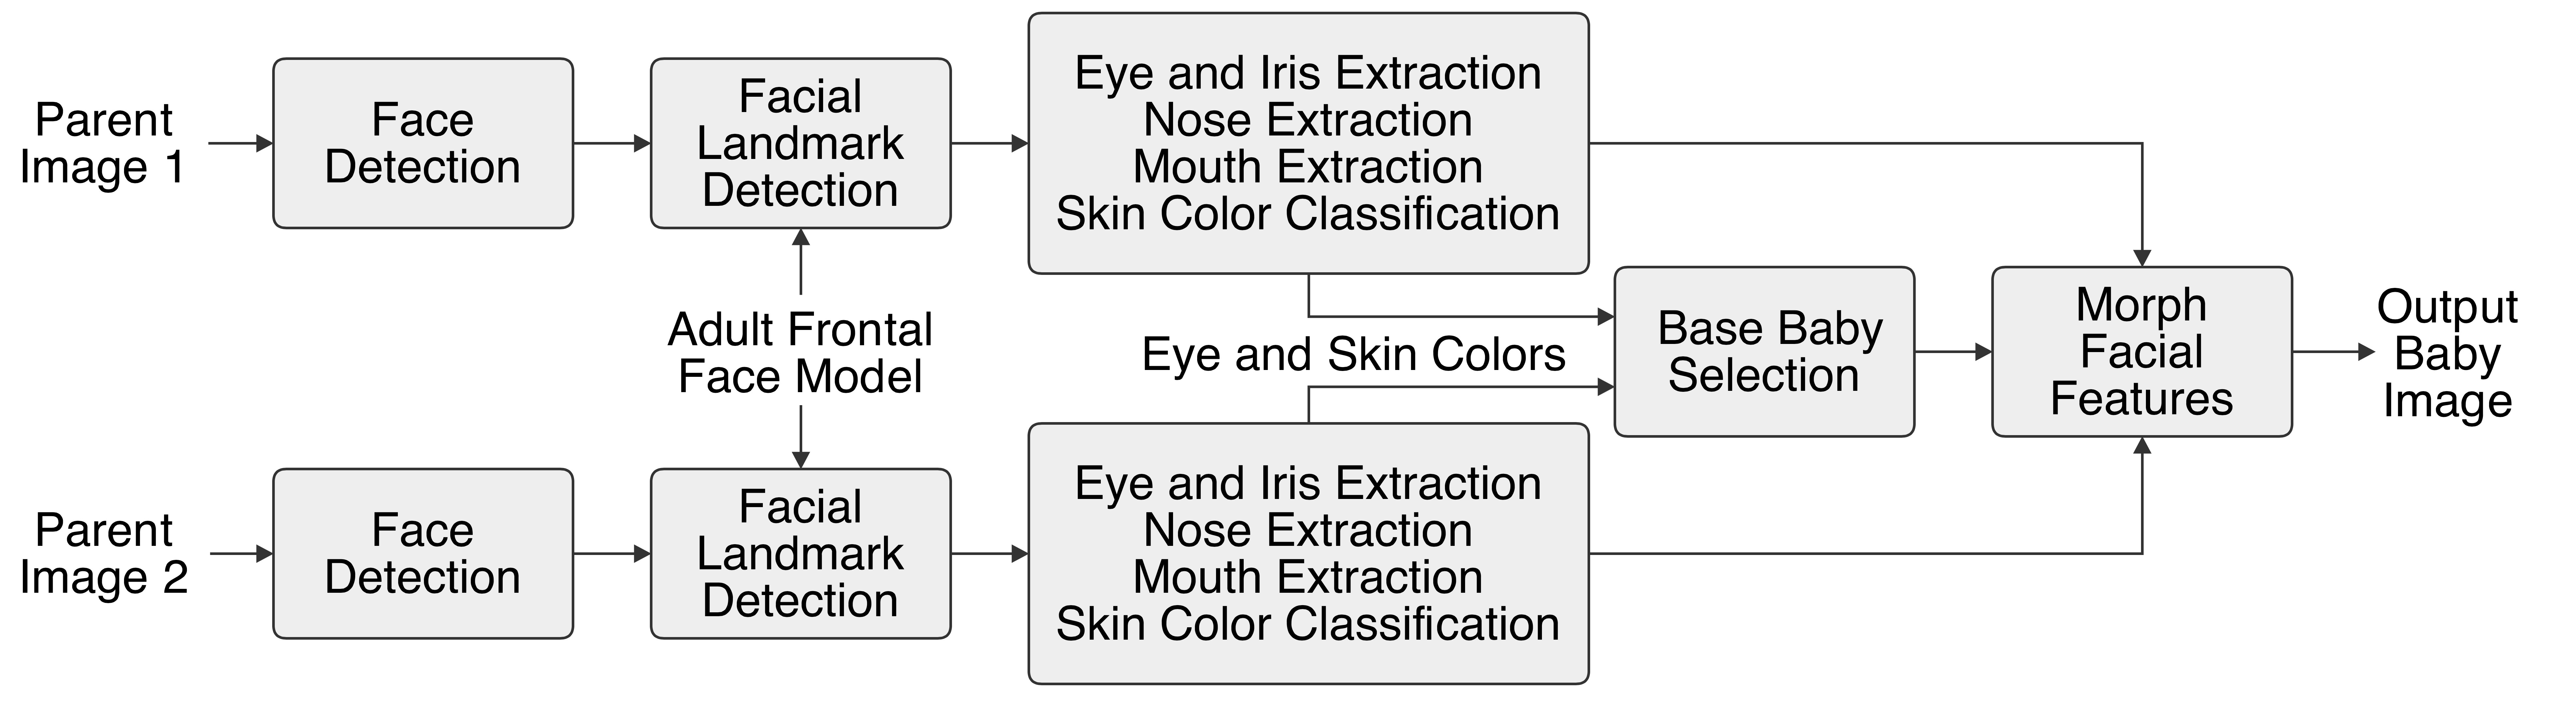
\includegraphics[scale=1]{Images/44}
    \end{center}
    \caption{Thuật toán tạo dưng khuôn mặt em bé}
    \label{refhinh1}
    \end{figure}
\end{center}

\begin{abstract}

Bài báo này giới thiệu một phương pháp để tạo ra khuôn mặt em bé từ hai hình ảnh bố mẹ. Các công đoạn đầu tiên bao gồm phát hiện khuôn mặt, nhận diện điểm mốc và trích xuất đặc trưng, nhằm thu thập thông tin liên quan từ mỗi hình ảnh gốc. Sử dụng thông tin này, thuật toán morphing được thực hiện, bao gồm: phân tách đặc trưng thành các tam giác và tứ giác dựa trên các đặc trưng mấu chốt, thực hiện warping trên các tam giác và chữ nhật dùng biến đổi affine và homography, và cross-dissolving các hình đã warping. Các đặc trưng hỗn hợp từ bố mẹ sau đó được kết hợp với các tính năng cơ bản của em bé và đặt vào khuôn mặt em bé tại các vị trí tương ứng.

\end{abstract}

\IEEEpeerreviewmaketitle

\section{GIỚI THIỆU}

Việc xác định, phân tích và chỉnh sửa các hình ảnh có chứa khuôn mặt người vẫn là một lĩnh vực nghiên cứu đang hoạt động, bao hàm nhiều kỹ thuật xử lý ảnh. Một lĩnh vực con của lĩnh vực nghiên cứu này, kỹ thuật tự động phát hiện và trích xuất đặc trưng từ khuôn mặt, được ứng dụng phổ biến, từ phân tích biểu hiện khuôn mặt đến bảo mật riêng tư trong ứng dụng Google Street View \cite{ref:r1}. Một lĩnh vực con khác, kỹ thuật morphing khuôn mặt, cũng có một loạt các ứng dụng bao gồm nhận diện khuôn mặt, kết hợp hài hước hai khuôn mặt. Mục đích của bài báo này là thúc đẩy hai lĩnh vực trên cho ứng dụng giải trí, bằng việc chuyển đổi thông minh hai bức ảnh bố mẹ để tạo ra khuôn mặt em bé.

Thuật toán được sử dụng để tạo khuôn mặt em bé, xem Hình 1, bao gồm ba thành phần chính: trích xuất đặc điểm khuôn mặt, lựa chọn em bé cơ bản, và morphing khuôn mặt. Các phần từ II đến IV thảo luận về các phương pháp và việc thực hiện cụ thể. Việc triển khai hệ thống tổng thể bao gồm một Giao diện đồ hoạ người dùng (GUI) của MATLAB, xem Hình 2, cho phép người dùng dễ dàng lựa chọn các hình ảnh từ file hoặc chụp nhanh bằng webcam và chạy mã morphing.

\section{TRÍCH XUẤT ĐẶC TRƯNG KHUÔN MẶT}
Bước đầu tiên để trích xuất đặc trưng khuôn mặt cho mỗi ảnh bố mẹ bao gồm việc phát hiện khuôn mặt dùng bộ dò Viola-Jones được cung cấp trong thư viện OpenCV \cite{ref:r2}. Đối với mỗi ảnh bố mẹ, các điểm mốc trên khuôn mặt (góc mắt, góc miệng và đầu mũi) được phát hiện bằng flandmark, một bộ dò có mã nguồn mở \cite{ref:r3}. Khung bao và các điểm mốc của khuôn mặt sau đó được sử dụng để tính bổ sung cho các điểm mấu chốt, xem Hình 3. Chi tiết xem trong phần Phụ lục A. Những điểm mấu chốt này được kết hợp với bộ dò biên để trích xuất đặc trưng của mỗi khuôn mặt, được diễn giải trong Phần II-A đến II-D.
\begin{center}
    \begin{figure}[!t]
    \begin{center}
     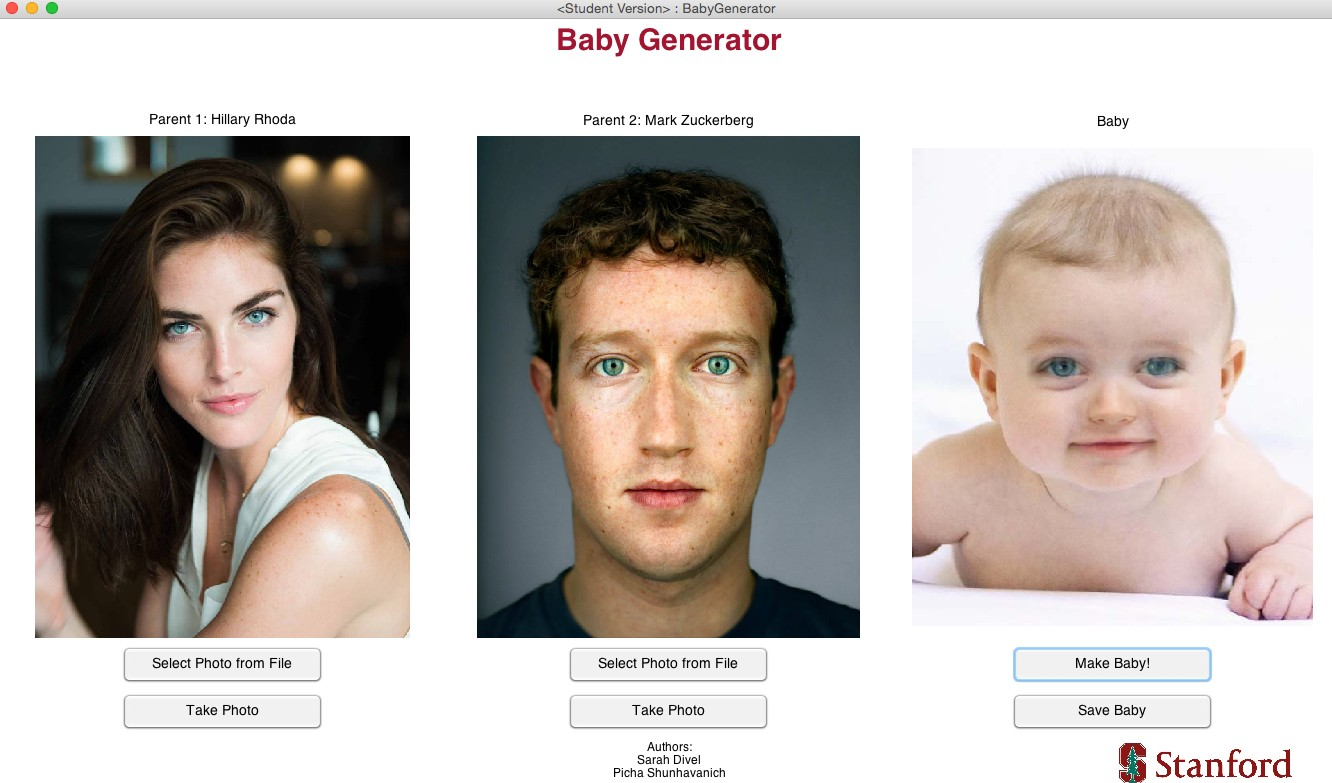
\includegraphics[scale=1]{Images/11}
    \end{center}
    \caption{Giao diện chương trình tạo dưng khuôn mặt em bé}
    \label{refhinh2}
    \end{figure}
    \begin{figure}[!t]
    \begin{center}
     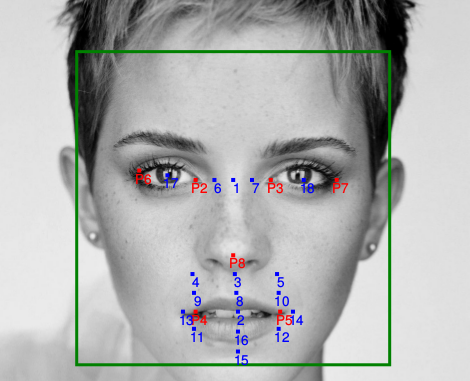
\includegraphics[scale=0.4]{Images/64}
    \end{center}
    \caption{Khung viền khuôn mặt(xanh lá),các điểm mốc(đỏ), các điểm mấu chốt(xanh dương)}
    \label{refhinh3}
    \end{figure}
\end{center}
\subsection{Mũi}

Việc trích xuất mũi chỉ cần dựa vào vùng hình thang tạo thành từ các điểm mấu chốt 4, 5, 7 và 6 theo ngược chiều kim đồng hồ. Sự lựa chọn này đến từ hai nhận xét: (1) những điểm mốc và điểm mấu chốt xung quanh mũi được phát hiện với độ chính xác cao và (2) mũi không có cạnh sắc bén nào khác ngoài lỗ mũi do đó việc phát hiện cạnh cho thêm thông tin giới hạn. Kết quả trích xuất mũi xem Hình 4b và Hình 4g.

\begin{figure}[!t]
\centering
\subfigure[Mắt thường]{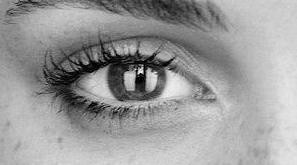
\includegraphics{Images/21}}
\subfigure[Mắt sau khi tái cấu trúc]{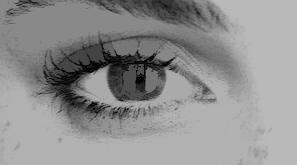
\includegraphics{Images/48}}
\subfigure[Đường biên mắt]{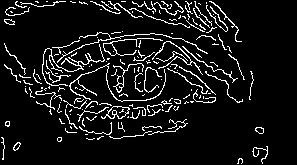
\includegraphics{Images/59}}
\subfigure[Trích xuất tròng mắt]{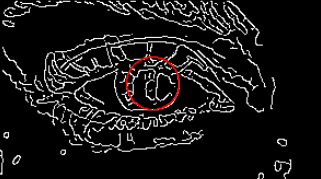
\includegraphics[scale=0.375]{Images/65}}
\subfigure[Mặt nạ]{
\includegraphics{Images/57}}
\subfigure[Mặt nạ đã loại bỏ sự phản chiếu]{
\includegraphics{Images/36}}
\caption{Trích xuất tròng mắt và màu mắt}
\label{refhinh5}
\end{figure}

\subsection{Mắt}

Việc trích xuất đặc trưng của mắt bao gồm trích xuất hình dạng mắt cũng như màu mắt. Bước đầu tiên trong trích xuất mắt là tìm kiếm vị trí và bán kính tròng mắt. Thuật toán phát hiện tròng mắt, dựa trên \cite{ref:r4}, là sự kết hợp của các kỹ thuật tái tạo hình thái (morphological reconstruction), phát hiện cạnh dùng bộ dò biên Canny [6], và phát hiện hình tròn dùng biến đổi Hough hình tròn. Bước đầu tiên trong thuật toán gồm việc trích xuất một khung bao lớn chứa con mắt được chọn và chuyển đổi vùng này sang ảnh xám. Việc tái tạo hình thái sau đó được dùng để trám các ánh phản chiếu trong mắt. Bộ dò biên Canny được dùng để tìm ra các biên. Một biến đổi vòng tròn Hough được tính toán trên biên ảnh để phát hiện ba vòng tròn nổi bật nhất [7]. Tâm của mỗi vòng tròn sau đó được so sánh với trung điểm tính từ hai vị trí góc mắt. Vòng tròn tròng mắt được chọn là vòng tròn có tâm gần nhất với trung điểm.

Để xác định màu mắt, mặt nạ của vòng tròn tròng mắt được áp dụng để trích xuất toàn bộ tròng mắt. Thêm vào đó, mặt nạ của ánh phản chiếu được xây dựng dựa trên sự chênh lệch ngưỡng giữa ảnh mắt gốc và ảnh tái tạo. Sử dụng mặt nạ này, trích xuất được các màu HSV (hue, saturation, value) của mắt. Cách tiếp cận này đưuọc minh hoạ trong Hình 5.

Sử dụng các điểm gốc góc, trung tâm tròng mắt, và bán kính mống mắt, tính được mặt nạ của hình dạng mắt bằng cách kết hợp hai mặt nạ hình ellipse. Do mắt thường có khoảng cách khác nhau từ điểm góc đến phần trên và phần dưới của mắt, việc dùng hai ellipse giúp điều tiết sự khác biệt này bằng cách cho phép khác biệt về bán kính trục nhỏ. Bán kính trục lớn của hai ellipse được tính bằng một nửa khoảng cách giữa vị trí $(0,98X_{left\, corner},\, Y_{left\, corner})$ và vị trí $(1.02X_{right\, corner}, \, Y_{right\,corner})$. Bán kính trục nhỏ của ellipse trên được tính bằng $1.2(r_{iris}+(y_{eye\,center}-y_{iris\,center}))$ và bán kính trục nhỏ của ellipse dưới được tính bằng $1.2(r_{iris}+(y_{eye\,center}-y_{iris\,center}))$ với $r_{iris}$ là bán kính của tròng mắt. Đường ranh giới giữa các ellipse được tính bằng đường nối giữa hai góc mắt. Một ví dụ về việc tạp mặt nạ cho mắt trái được thể hiện trong Hình 6. Kết quả của việc trích xuất mắt xem trong Hình 4c-d và Hình 4h-i.
\begin{figure}[!t]
\centering
\subfigure[Mắt thường]{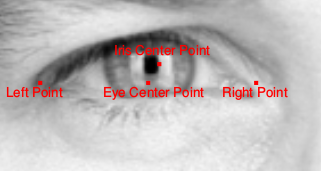
\includegraphics[scale=0.38]{Images/66}}
\subfigure[Combined Eye Ellipse Mask]{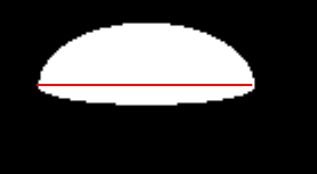
\includegraphics[scale=0.38]{Images/67}}
\subfigure[Lower Ellipse with Dividing Line]{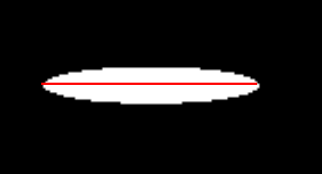
\includegraphics[scale=0.38]{Images/68}}
\subfigure[Upper Ellipse with Dividing Line]{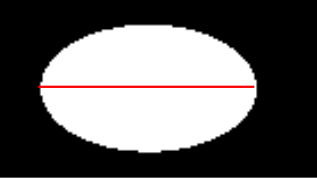
\includegraphics[scale=0.38]{Images/70}}
\caption{Trích xuất hình ảnh mắt}
\label{refhinh6}
\end{figure}

\begin{figure*}[!t]
\centering
\subfigure[Emma Watson]{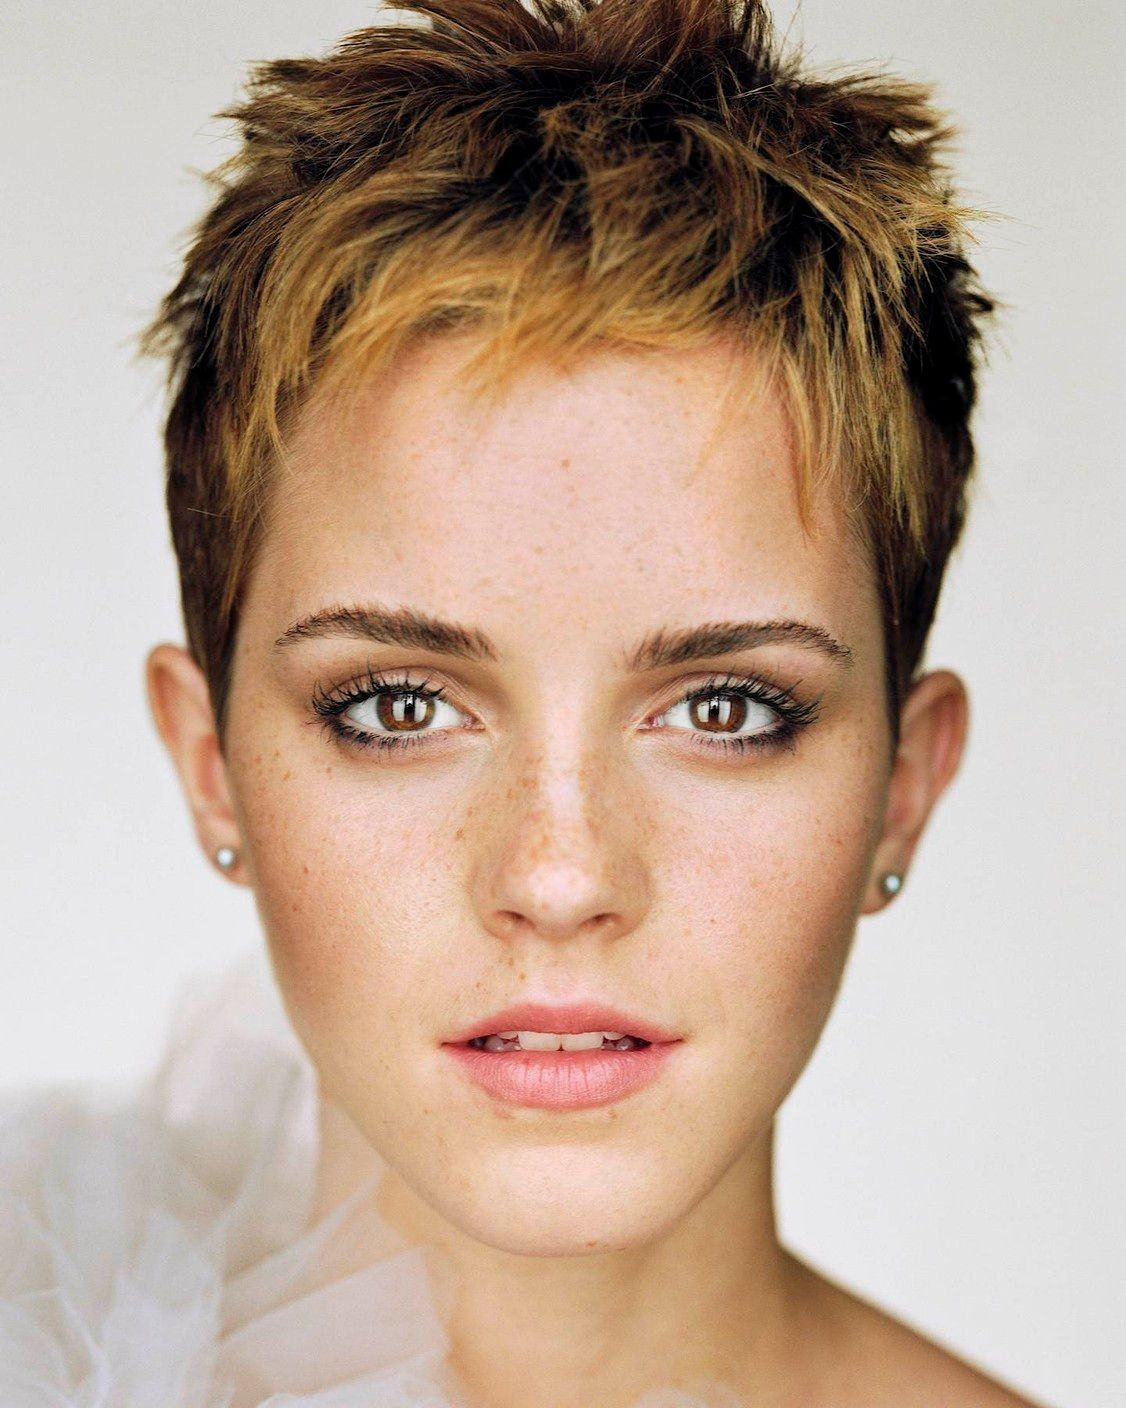
\includegraphics{Images/35}}
\subfigure[Mũi Emma Watson]{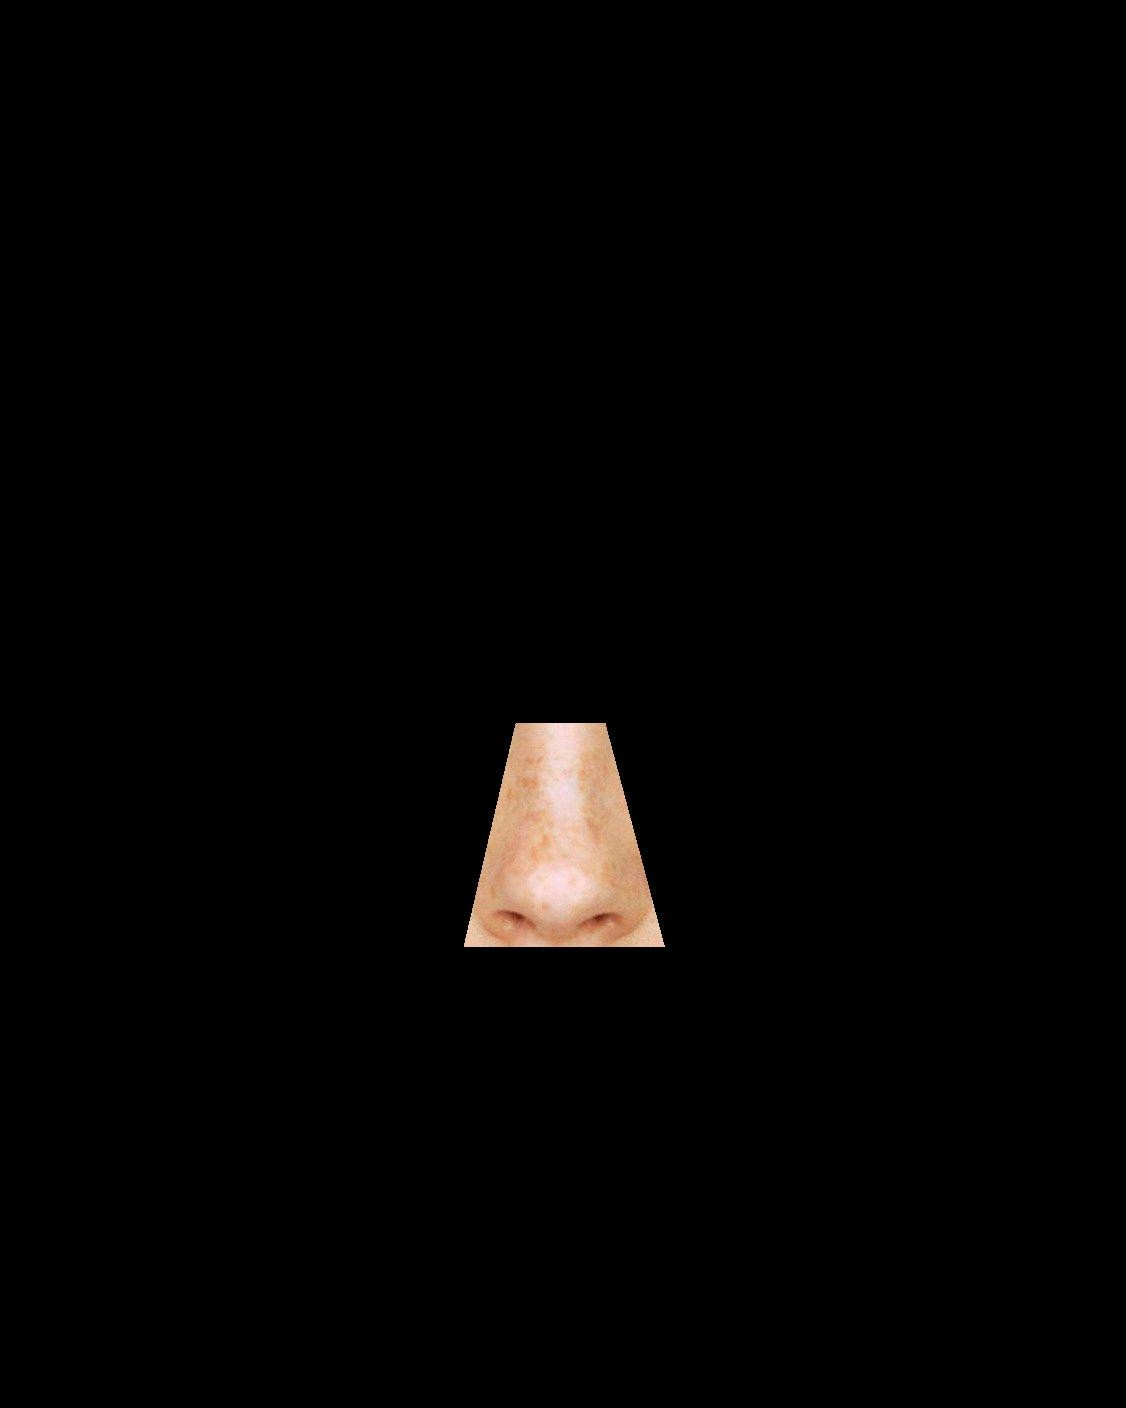
\includegraphics{Images/41}}
\subfigure[Mắt phải Emma Watson]{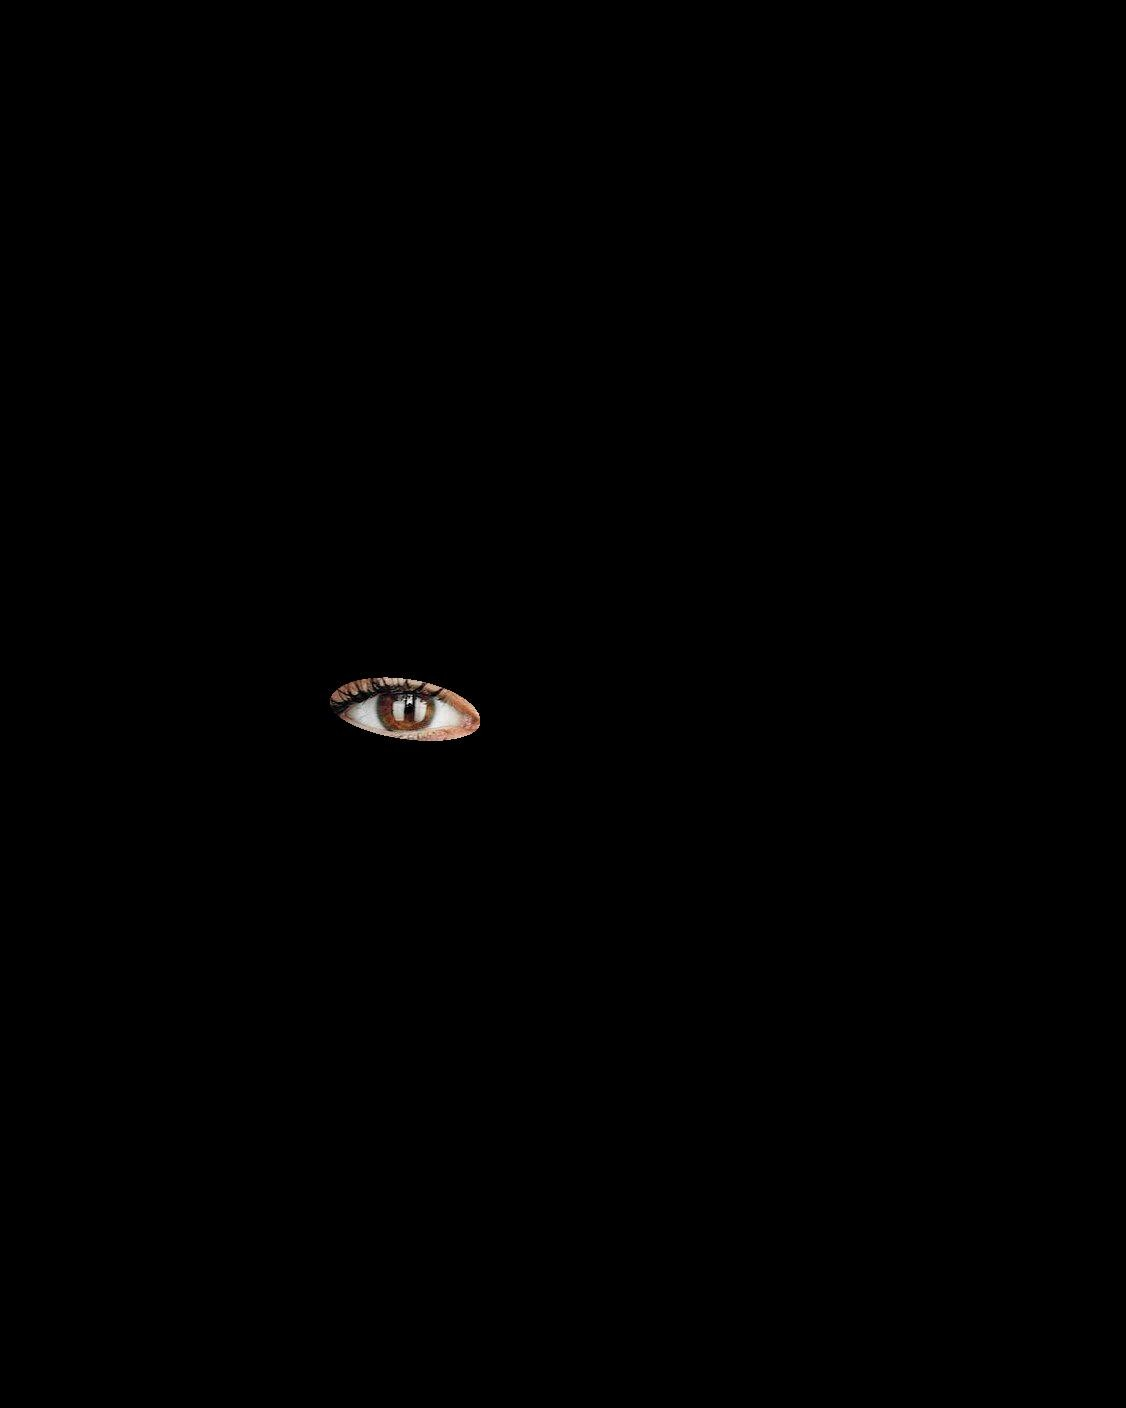
\includegraphics{Images/9}}
\subfigure[Mắt trái Emma Watson]{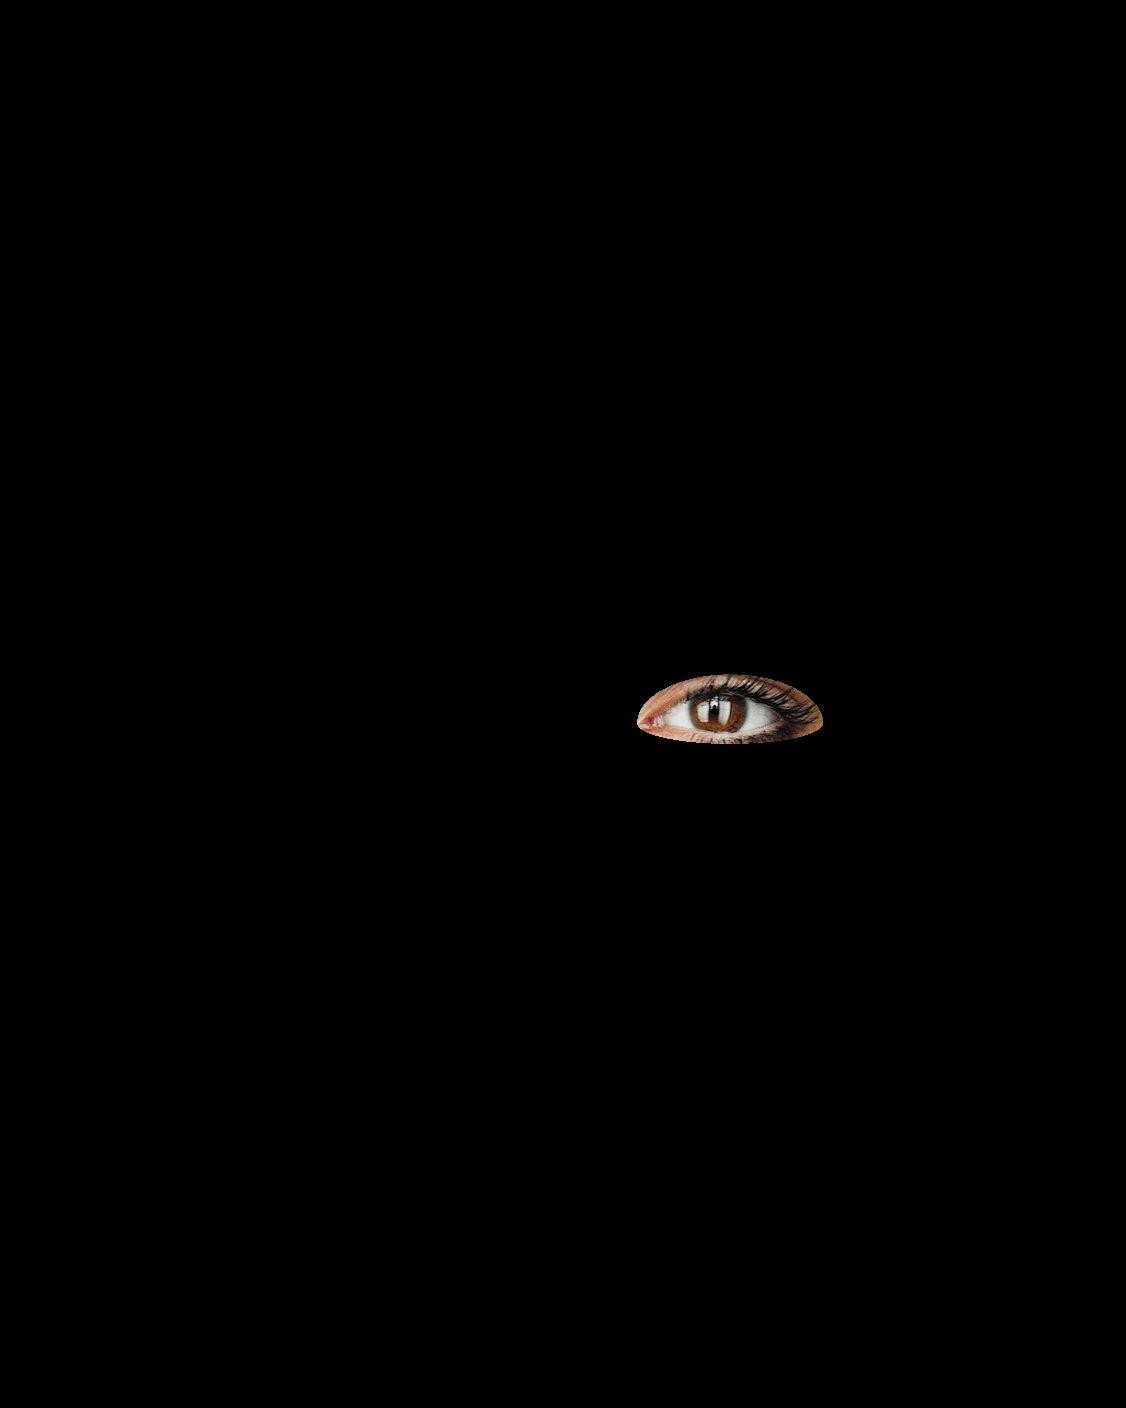
\includegraphics{Images/8}}
\subfigure[Miệng Emma Watson]{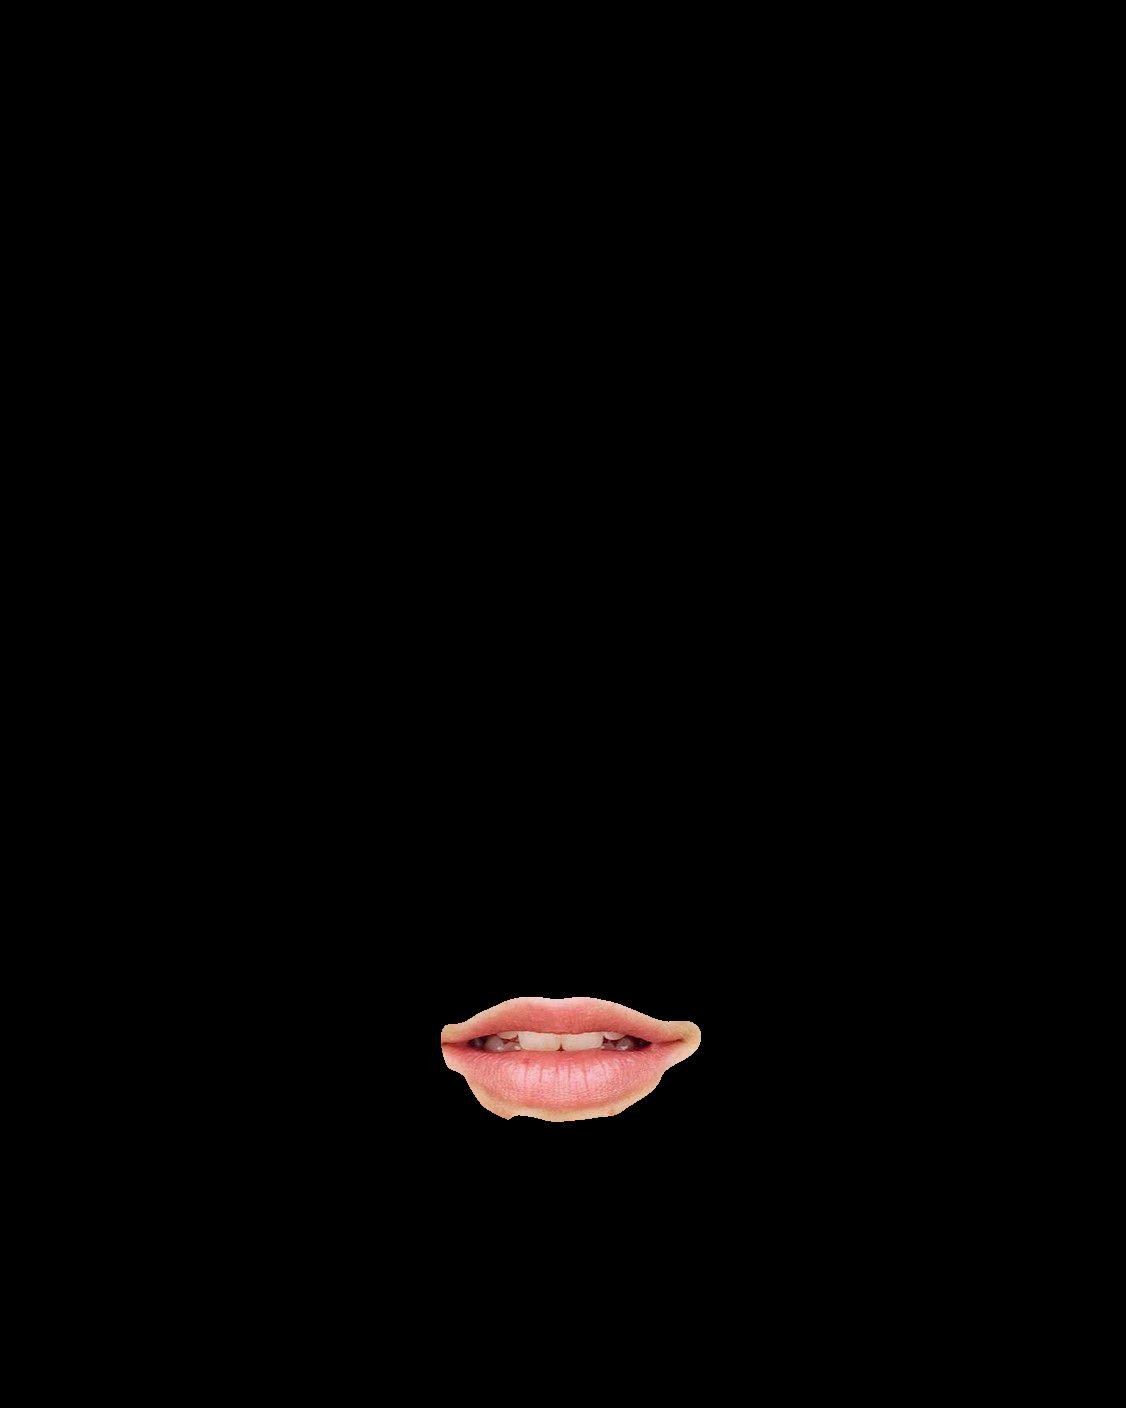
\includegraphics{Images/32}}
\subfigure[Ben Affleck]{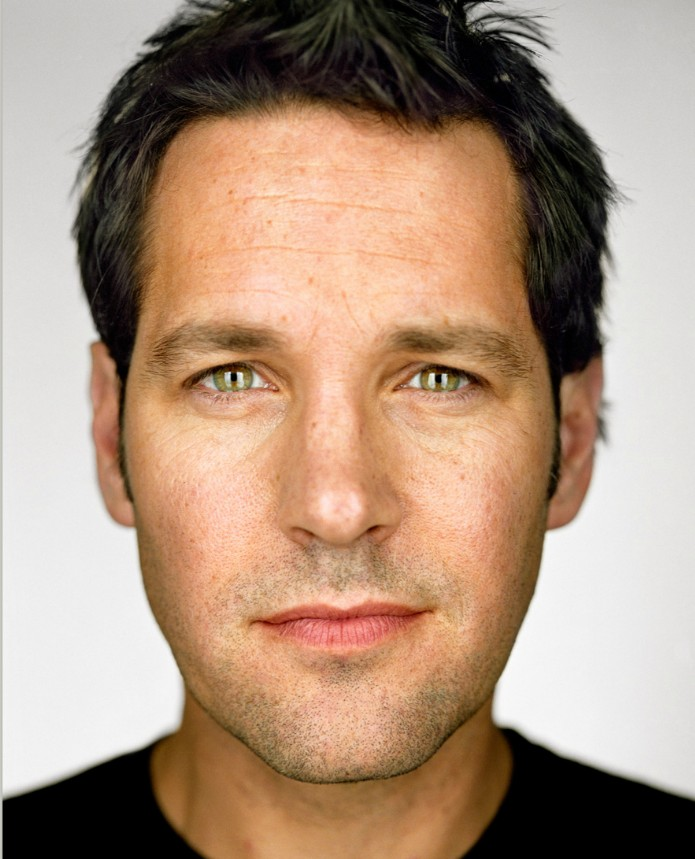
\includegraphics{Images/29}}
\subfigure[Mũi Ben Affleck]{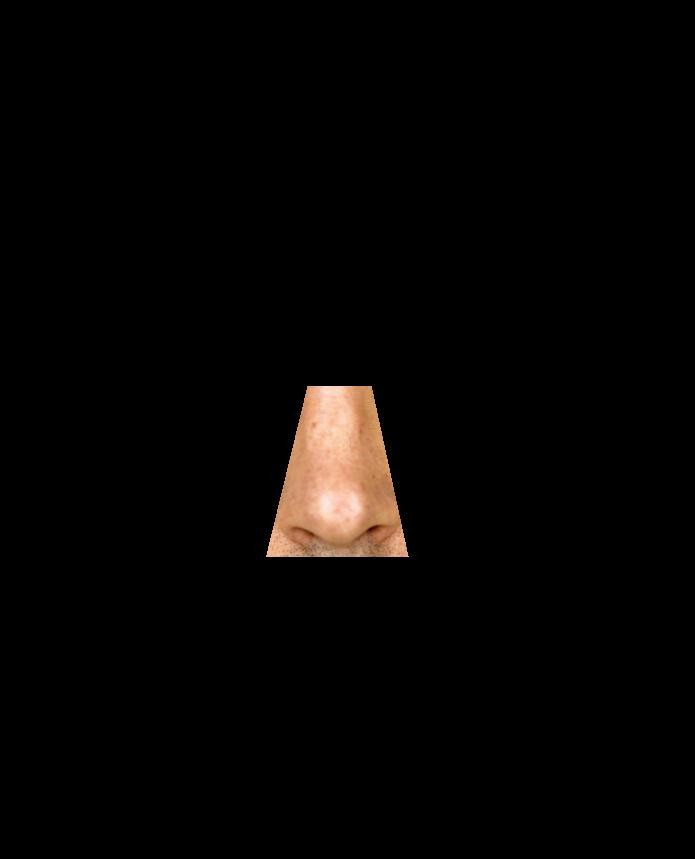
\includegraphics{Images/34}}
\subfigure[Mắt phải Ben Affleck]{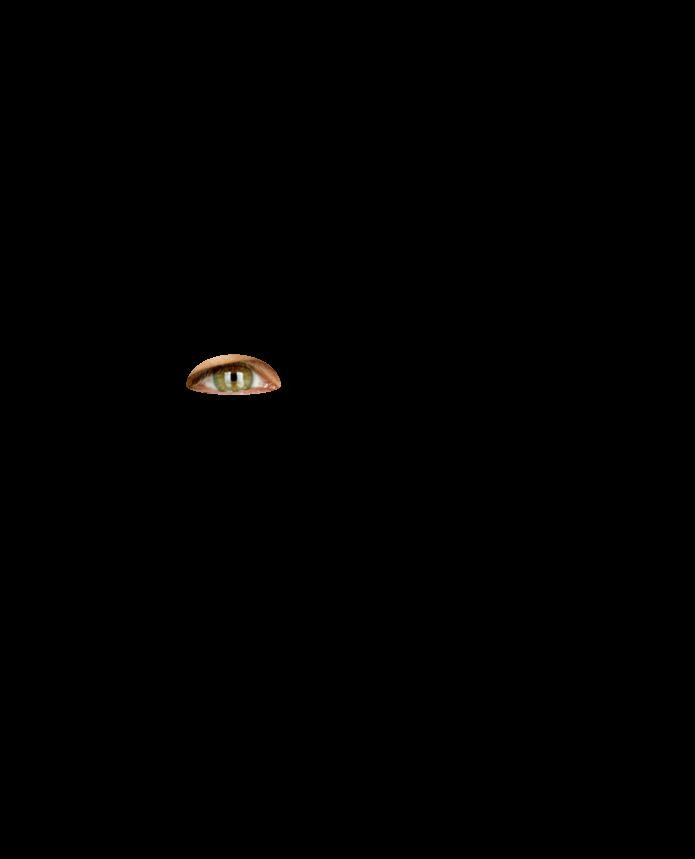
\includegraphics{Images/26}}
\subfigure[Mắt trái Ben Affleck]{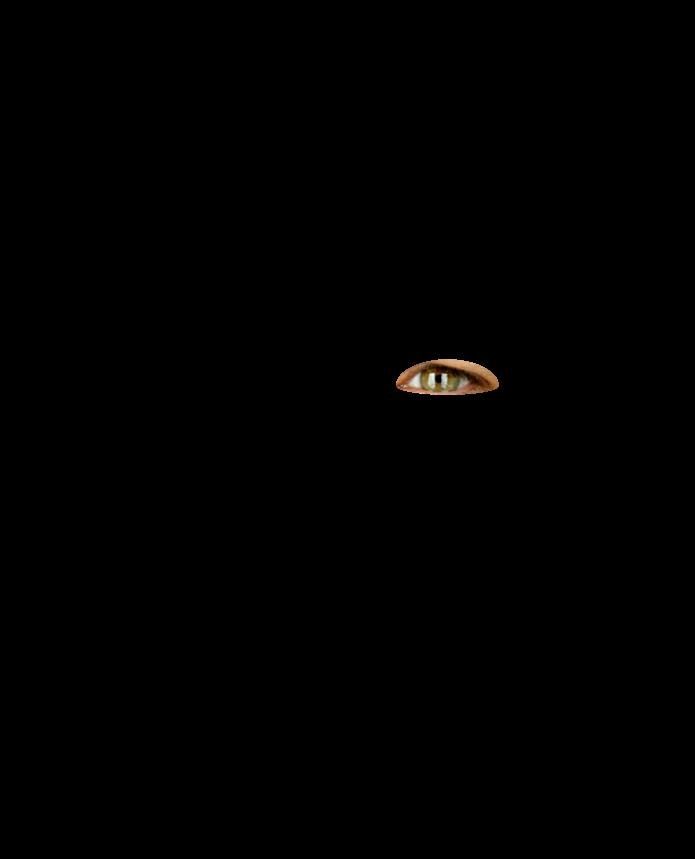
\includegraphics{Images/24}}
\subfigure[Miệng Ben Affleck]{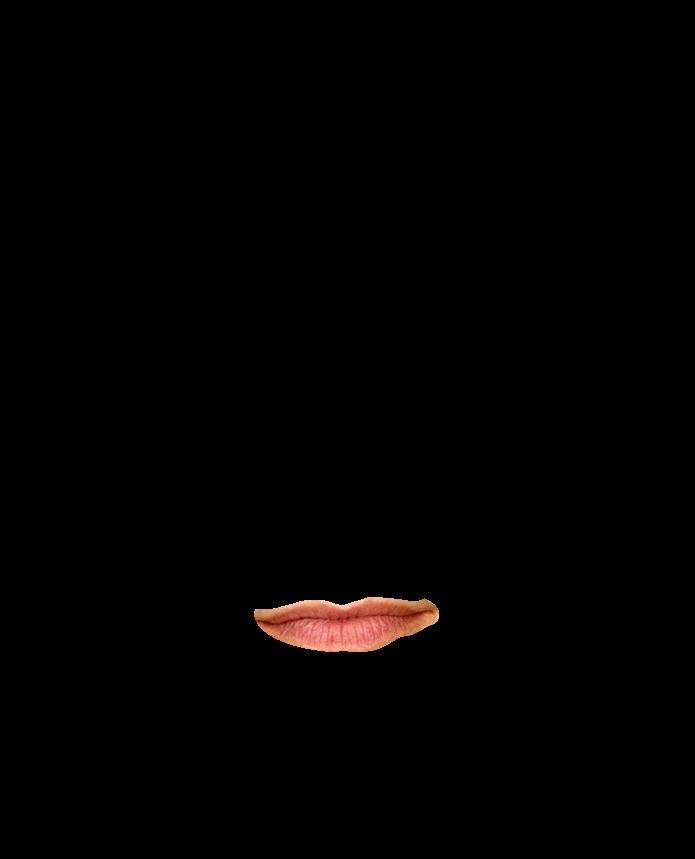
\includegraphics{Images/51}}
\caption{Trích xuất đặc trưng khuôn mặt}
\label{refhinh4}
\end{figure*}

\subsection{Miệng}
Một quy trình hai bước được thực hiện để trích xuất miệng của từng ảnh bố mẹ. Đầu tiên là phương pháp được diễn giải trong Phần II-B, dùng hai mặt nạ ellipse để trích xuất mặt nạ tổng quát cho miệng. Phần thứ hai của thuật toán để gồm việc phát hiện biên trên một ảnh tăng cường-môi (lip-enhanced). Phép chuyển đổi từ hệ màu RGB sang hệ màu tăng cường-môi được mô tả bởi công thức $14(2G-R-0.5B)$ iúp nâng cao mức thành công của bộ dò biên môi, vì nó phân biệt rõ màu da và môi, như Hình 7. Việc phát hiện cạnh sử dụng toán tử Laplacian của Gaussian đã được thực hiện trên ảnh tăng cường-môi như Hình 7.
\begin{figure}[!h]
\centering
\subfigure[Lip-enhanced image]{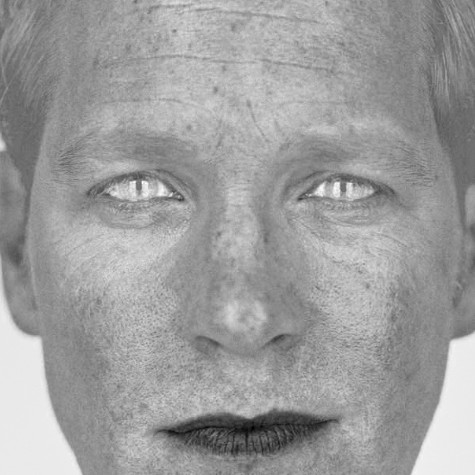
\includegraphics{Images/63}}
\subfigure[Edges detected]{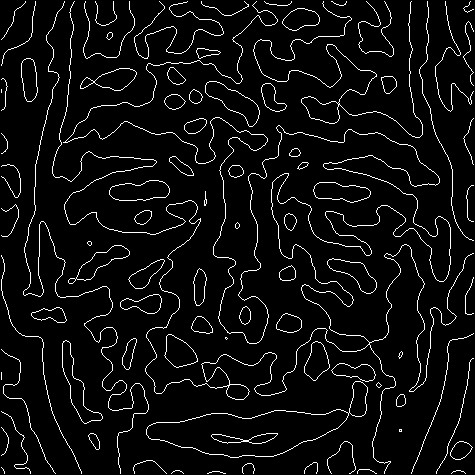
\includegraphics{Images/61}}
\subfigure[Mouth mask based on lip edges]{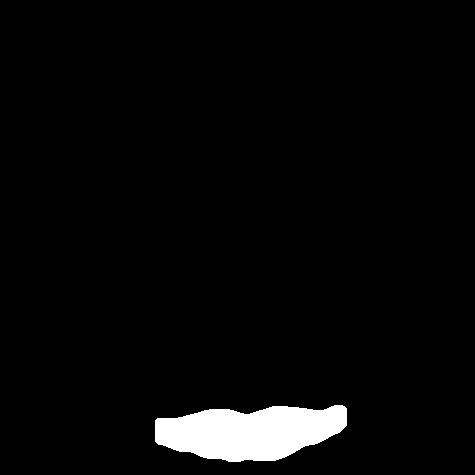
\includegraphics{Images/13}}
\subfigure[Combined mouth masks]{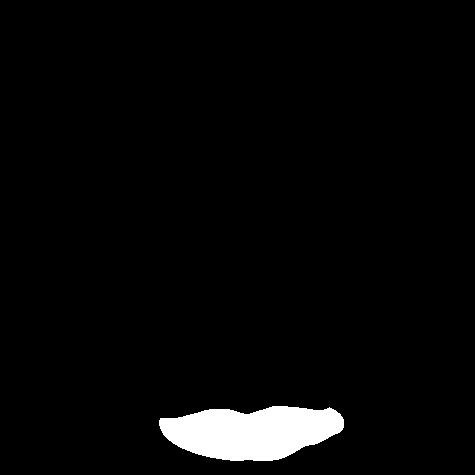
\includegraphics{Images/30}}
\caption{Trích xuất miệng}
\label{refhinh7}
\end{figure}
Kế đến, thực hiện tìm biên gần nhất với các điểm mốc của miệng, P4 và P5. Nếu biên gần nhất với P4 giao với biên gần nhất với P5, nó được xác định là biên môi. Nếu điều kiện này không thoả, mặt nạ biên bị loại bỏ và chỉ có hai mặt nạ ellipse được sử dụng.

Để tạo ra mặt nạ biên cho miệng, biên của môi được làm đầy và sau đó mở rộng một chút để đảm bảo môi không bị cắt. Hai mặt nạ ellipse được phủ lên mặt nạ biên miệng để tạo ra mặt nạ miệng cuối cùng. Kết quả của việc trích xuất miệng xem trong Hình 4e và Hình 4j.


\begin{figure}[!t]
\centering
\subfigure[Original facial bounding box of
Hillary Rhoda]{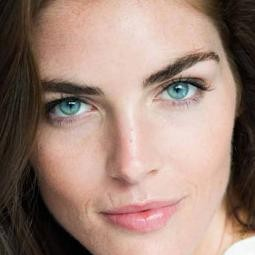
\includegraphics{Images/12}}
\subfigure[Skin regions detected]{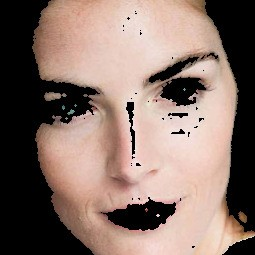
\includegraphics{Images/3}}
\caption{Trích xuất vùng da}
\label{refhinh8}
\end{figure}

\subsection{Da}
Màu da là đặc trưng cuối cùng được trích xuất từ ảnh bố mẹ và dựa trên việc phân đoạn màu da thành 6 khúc trên hệ màu HSV [9]. Sử dụng việc phân đoạn trong hệ màu HSV này, vùng da trên khuôn mặt được xác định và được dùng để tính các giá trị HSV trung bình cho màu da của bố mẹ. Kết quả tạo mặt nạ da có thể xem trong Hình 8.



\section{ẢNH GỐC EM BÉ}
Bộ cơ sở dữ liệu bao gồm ảnh của chín em bé với màu da và màu mắt khác nhau sẽ được so sánh và chọn lọc dựa trên những đặc điểm tương đồng với hình ảnh của bố mẹ. Vì thư viện flandmark dựa trên hình mẫu khuôn mặt của người lớn, mà hình dạng của khuôn mặt trẻ em lại rất khác với giữa người lớn, nên việc định vị các điểm mốc của khuôn mặt phải được thực hiện thủ công. Các điểm mấu chốt trên khuôn mặt sẽ được tính toán bằng các phương trình hiệu chỉnh để phù hợp với khuôn mặt em bé. Sau cùng, các đặc trưng sẽ được trích xuất bằng phương pháp được trình bày ở mục II-A tới II-D. 

\begin{figure}[!t]
\centering
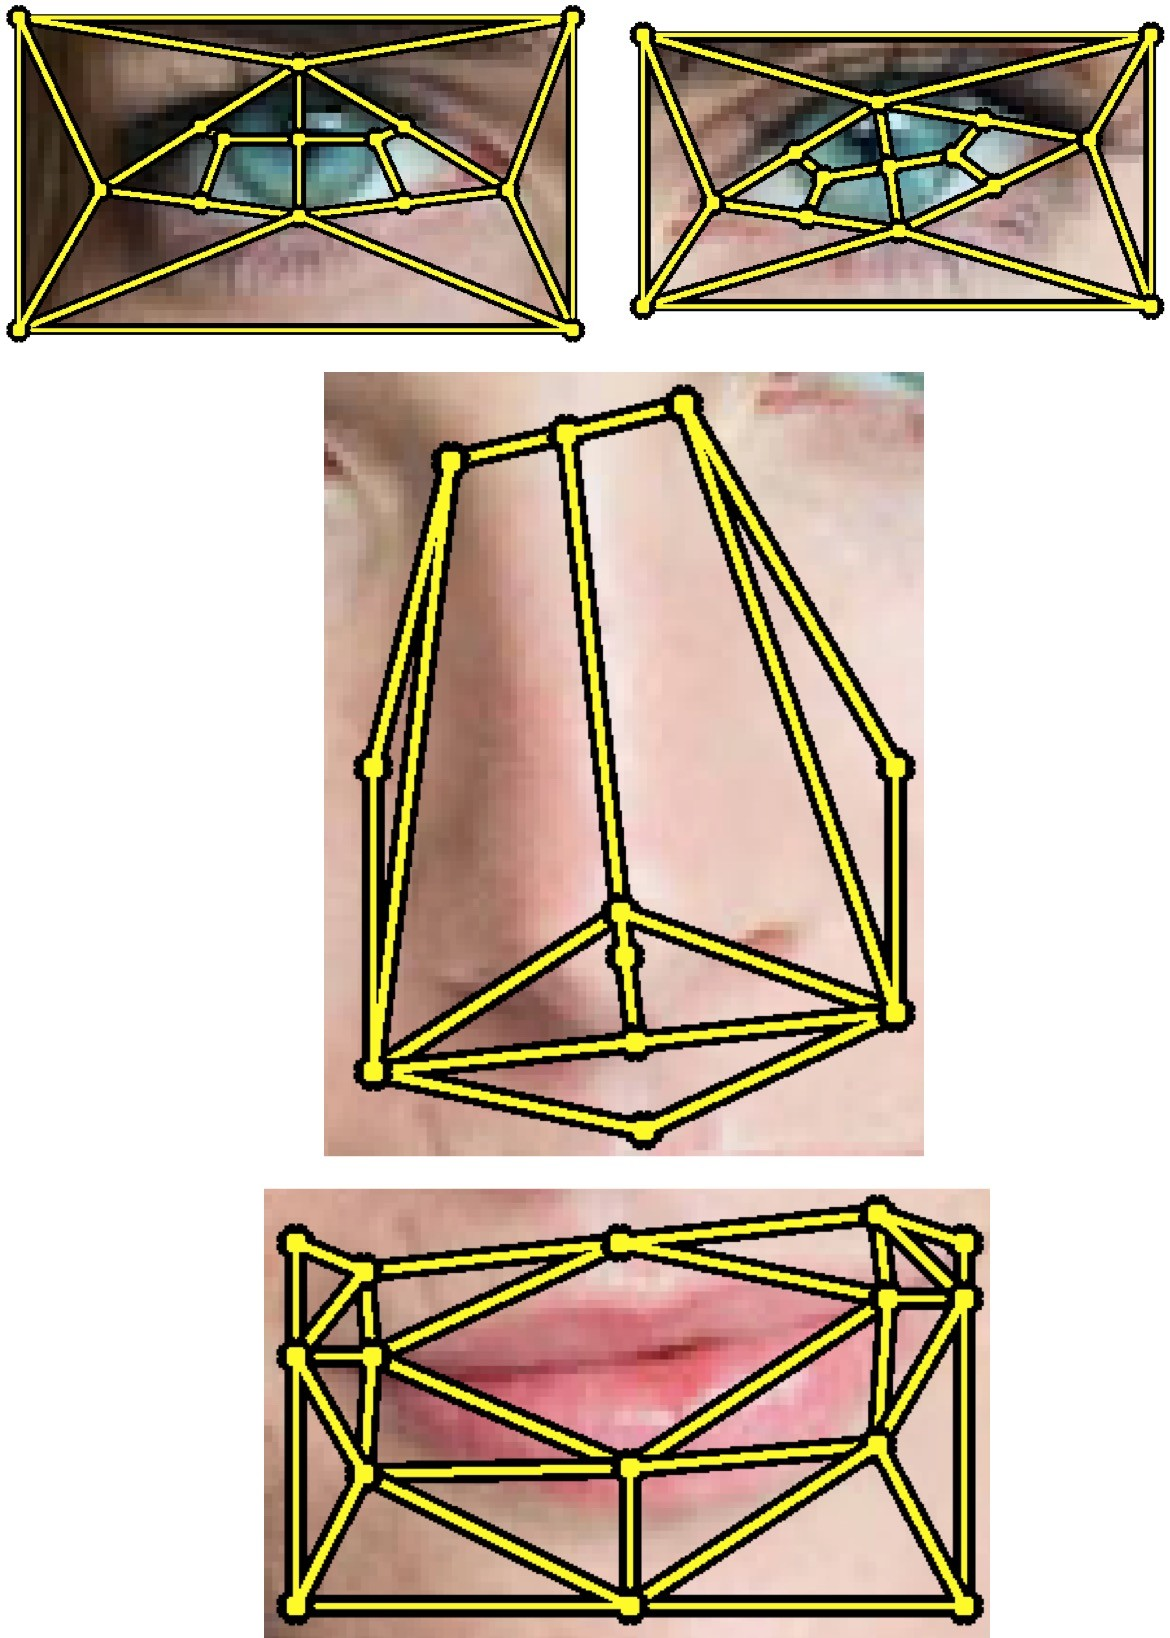
\includegraphics{Images/17}
\caption{Phân vùng các đặc tính khuôn mặt của Hillary Rhoda}
\label{refhinh9}
\end{figure}

Để chọn được tấm ảnh gốc em bé phù hợp với hình ảnh cha mẹ, yếu tố căn bản cần xem xét là màu da. Việc so sánh được thực hiện bằng cách tổ hợp tuyến tính các giá trị HSV (hue, saturation, value) của màu da bố và mẹ để tạo ra màu da tổng hợp, rồi chọn ra ảnh gốc em bé có màu da trong hệ màu HSV gần nhất với màu da tổng hợp này. Ngoài ra nếu cả bố và mẹ đều có mắt xanh lá hoặc xanh dương, ảnh em bé với màu mắt đó sẽ được chọn.

\section{MORPHING CÁC ĐẶC TÍNH}
Các đặc trưng khuôn mặt (mắt, mũi và miệng) được kết hợp từ bố, mẹ, và ảnh gốc em bé bằng một thuật toán morphing dựa trên thuật toán mesh warping [10], [11]. Thuật toán này trải qua 4 giai đoạn: phân vùng ảnh, warping, cross dissolving, và tạo dựng hình ảnh em bé.
\subsection{Phân tách ảnh}
Mỗi đặc trưng khuôn mặt trước hết được phân tách thành các tam giác hoặc tứ giác dựa trên các điểm mấu chốt đã được trích xuất (xem Hình 9).
\subsection{Warping}
Các đặc trưng khuôn mặt từ bố mẹ được trích xuất ra như ở hình A và B. Hình A được warping thành A0, và hình B được được warping thành B0 để cả hai có cùng kích cỡ và hình dạng. Hình dạng này được tính toán bằng phương pháp nội suy tuyến tính các điểm tương đương trên lưới giữa hình A và B. Trong quá trình warping, một phép biến đổi affine được sử dụng để ánh xạ tọa độ của các tam giác từ ảnh gốc sang ảnh được warping, trong khi đó phép homography sẽ được áp dụng cho các tứ giác. Phương trình của phép biến đổi tọa độ là:\[\textbf{\underline{x}'} = T\textbf{\underline{x}}\] 
Với \textbf{\underline{x}} và \textbf{\underline{x}'} lần lượt là tọa độ tương ứng, với dạng, với dạng $[x\; y\; 1]^T$  ủa ảnh gốc và ảnh được warping.
\\
Công thức biến đổi affine
\begin{align*}
	T =
    \begin{bmatrix}
        a_{1,1} & a_{1,2} & a_{1,3} \\
        a_{2,1} & a_{2,2} & a_{2,3} \\
        0 & 0 & 1
    \end{bmatrix}
\end{align*}
Công thức homography
\begin{align*}
	T =
    \begin{bmatrix}
        a_{1,1} & a_{1,2} & a_{1,3} \\
        a_{2,1} & a_{2,2} & a_{2,3} \\
        a_{3,1} & a_{3,2} & a_{3,3}
    \end{bmatrix}
\end{align*}

\begin{figure}[!t]
\centering
\subfigure[A]{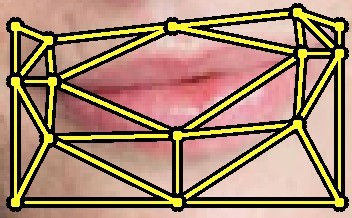
\includegraphics[scale=0.97]{Images/16}}
\subfigure[B]{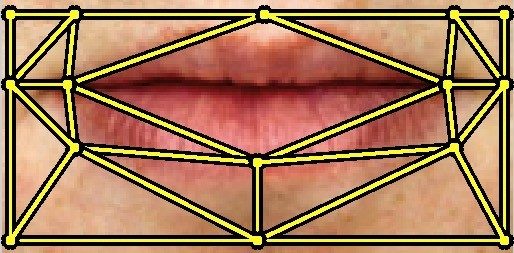
\includegraphics{Images/22}}
\subfigure[A']{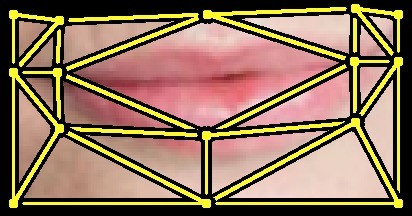
\includegraphics{Images/31}}
\subfigure[B]{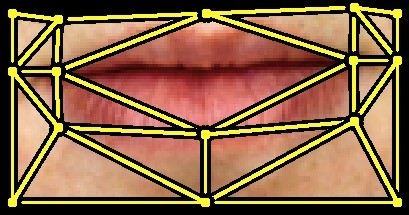
\includegraphics{Images/43}}
\subfigure[Cross-dissolving của A' và B', I]{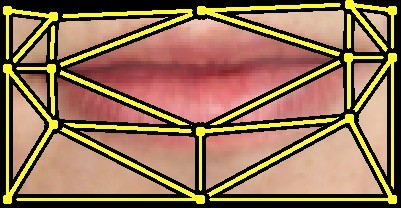
\includegraphics{Images/50}}
\label{refhinh10}
\caption{Morphing of two parent features, A and B}
\end{figure}
Quá trình trên ánh xạ toạ độ của các điểm ảnh trên ảnh đích đến các điểm ảnh trên ảnh gốc, rồi gán màu sắc nội suy của ảnh gốc cho ảnh đích, với \[\textbf{\underline{x}} = T^{-1}\textbf{\underline{x}'}\]
Điều này đảm bảo tất cả điểm ảnh trên ảnh đích đều được gán giá trị.

\subsection{Cross-Dissolving}
Sau khi hai ảnh đặc trưng được warping vào các vị trí trung gian tương ứng, chúng được cross-dissolving bằng cách tính toán trọng số trung bình của hai ảnh bằng công thức
\[I[x,y]=\alpha A'[x,y]+(1-\alpha) B'[x,y]\]
Với $0 < \alpha < 1$. Kết quả cross-dissolve từ hình của hai bố mẹ ở Hình 10c và Hình 10d được thể hiện ở Hình 10e.

\subsection{Tạo dựng hình ảnh em bé}
Các đặc trưng hỗn hợp của người lớn sẽ được morphing với các đặc trưng tương ứng trên ảnh gốc em bé sử dụng các bước morphing (phân vùng ảnh, warping, và cross-dissolving) như đã được miêu tả ở trên. Điều này là cần thiết để đảm bảo các đặc trưng sau cùng trông giống với một em bé, vì một số đặc trưng nhất định vốn rất khác nhau giữa trẻ em và người lớn. Ví dụ, trẻ em có tròng mắt lớn hơn và sống mũi phẳng hơn. Kết quả của phép warping cuối cùng này được thể hiện trong Hình 11.
\begin{figure}[!t]
\centering
\subfigure[Đặc tính hỗn hợp của khuôn mặt người lớn, I]{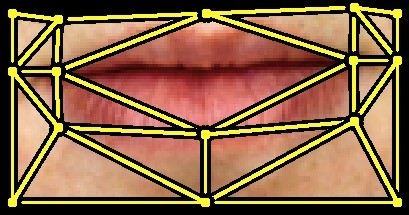
\includegraphics{Images/43}}
\subfigure[Đặc tính cơ bản của khuôn mặt em bé, C]{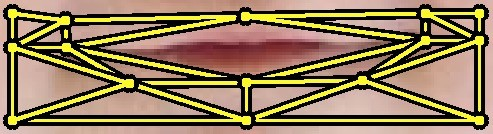
\includegraphics{Images/19}}
\subfigure[Đặc tính hỗn hợp của khuôn mặt người lớn đã được làm cong 	, I']{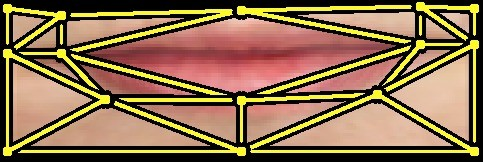
\includegraphics{Images/46}}
\subfigure[Đặc tính cơ bản của khuôn mặt em bé đã được làm cong, C']{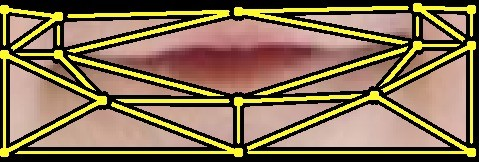
\includegraphics{Images/6}}
\subfigure[Cross-dissolving của I' và C', F]{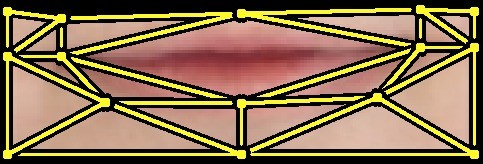
\includegraphics{Images/15}}
\label{refhinh11}
\caption{Morphing giữa đặc tính hỗn hợp của khuôn mặt người lớn và đặc tính cơ bản khuôn mặt em bé, A và B}
\end{figure}
Bước tiếp theo, các đặc trưng được tạo ra, F, sẽ được đặt chồng lên ảnh gốc em bé sao cho điểm trung tâm của các đặc trưng trùng nhau. Các điểm biên của vùng đặc trưng sẽ được làm mượt để làm cho các đặc trưng được tạo ra hòa lẫn vào vùng biên trên ảnh gốc em bé. Một mặt nạ nhị phân xung quanh F, BW, sẽ được tạo, sử dụng open filter và erode để làm cho mặt nạ nhị phân mượt hơn và nhỏ hơn. Một bộ lọc Gauss được áp dụng lên mặt nạ nhị phân để tạo ra mặt nạ trọng số $\sigma$. Dựa trên các đặc trưng khuôn mặt, ta có thể áp dụng bộ lọc trung bình hoặc bộ lọc Gauss lên nghịch đảo của BW nhằm tạo ra mặt nạ trọng số $\beta$. Hình 12 minh họa mặt nạ trọng số được sử dụng trong quá trình làm mượt ảnh.  

Các đặc tính đặc lên ảnh gốc em bé được tính toán theo công thức \[Feature = \beta I_{baby}+(1 - \beta )(\sigma F+(1-\sigma )C')\]
Trong đó $I_{baby}$ là ảnh em bé gốc.

Việc làm mượt với ảnh warping em bé là cần thiết vì đôi khi các đặc trưng gốc trên ảnh gốc em bé là rất khác so với các đặc trưng được tạo ra từ ảnh bố mẹ, khiến việc biến đổi trên đường viên gặp khó khăn. Ví dụ, ảnh gốc em bé có mũi rộng hơn nhiều so với mũi được tạo ra, khiến cho phần rìa của mũi em bé trên ảnh gốc vẫn xuất hiện trên ảnh đích nếu như sử dụng phương pháp gradual transition. Để giải quyết vấn đề này, ta sẽ trích xuất đặc trưng nhiều hơn trên vùng xung quanh của ảnh.

\begin{figure}[!t]
\centering
\subfigure[Mặt nạ trọng số $\sigma$ của mắt trái]{
\includegraphics{Images/60}}
\subfigure[Mặt nạ trọng số $\beta$ của mắt trái]{
\includegraphics{Images/18}}
\subfigure[Mặt nạ trọng số $\sigma$ của mắt phải]{
\includegraphics{Images/5}}
\subfigure[Mặt nạ trọng số $\beta$ của mắt phải]{
\includegraphics{Images/53}}
\subfigure[Mặt nạ trọng số $\sigma$ của mũi]{
\includegraphics{Images/55}}
\subfigure[Mặt nạ trọng số $\beta$ của mũi]{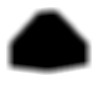
\includegraphics{Images/42}}
\subfigure[Mặt nạ trọng số $\sigma$ của miệng]{
\includegraphics{Images/23}}
\subfigure[Mặt nạ trọng số $\beta$ của miệng]{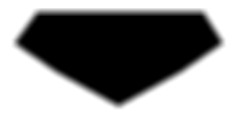
\includegraphics{Images/33}}
\label{refhinh12}
\caption{Mặt nạ trọng số dùng trong việc làm mượt ranh giới của mỗi đặc tính}
\end{figure}

\section{KẾT QUẢ}
Chương trình Tạo dựng Khuôn mặt Em bé được thử nghiệm trên 30 ảnh người lớn khác nhau. Kết quả phép thử được thể hiện trong Hình 13. Từ bài kiểm tra chất lương, các khuôn mặt em bé được tạo ra có các đặc trưng tương đối giống với cặp bố mẹ, đặc biệt là hình dáng mũi, miệng, màu mắt và màu da.

Tuy nhiên, nếu một trong hai ảnh bố hoặc mẹ được đưa vào nghiêng một góc lớn, khuông mặt được tạo ra sẽ trông không thật. Dù sao, chương trình có được thể thiết kế để chỉ chấp nhận ngõ vào là ảnh chụp thẳng khuôn mặt, vì mục đích của chương trình là tương tác trực tiếp với các người dùng.

\begin{figure}[!t]
\centering
\subfigure[Hình ảnh cha mẹ 1a]{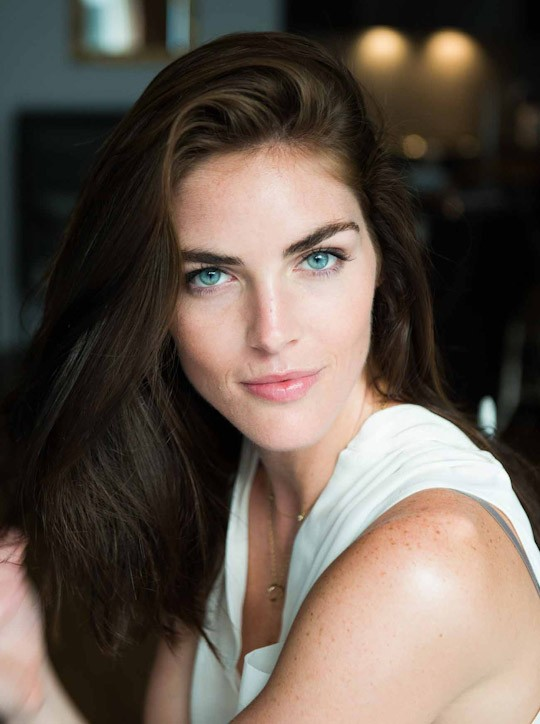
\includegraphics[scale=0.95]{Images/14}}
\subfigure[Hình ảnh cha mẹ 1b]{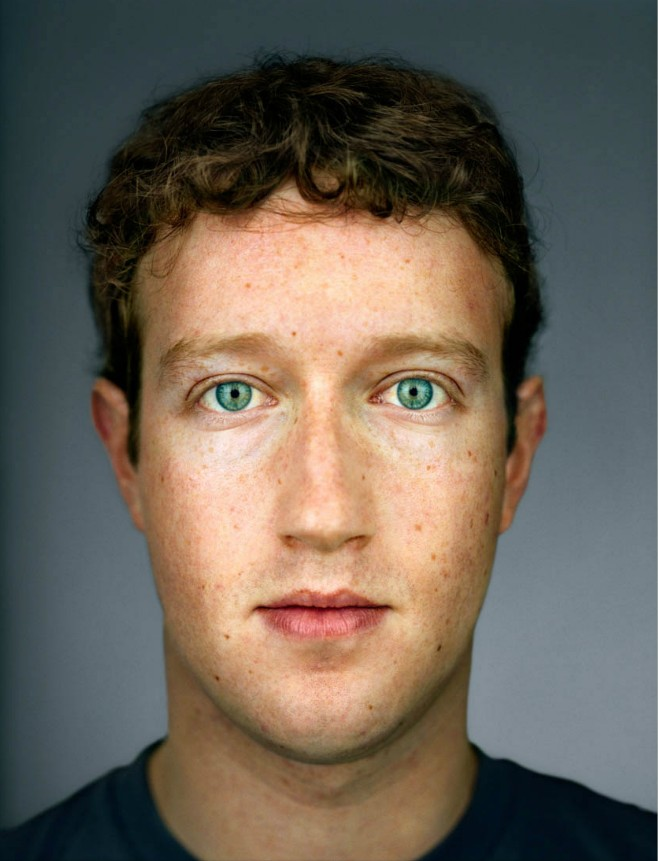
\includegraphics{Images/38}}
\subfigure[Hình ảnh em bé 1]{\includegraphics{Images/58}}
\subfigure[Hình ảnh cha mẹ 2a]{\includegraphics[scale=0.7]{Images/10}}
\subfigure[Hình ảnh cha mẹ 2b]{\includegraphics[scale=0.9]{Images/45}}
\subfigure[Hình ảnh em bé 2]{\includegraphics{Images/25}}
\subfigure[Hình ảnh cha mẹ 3a]{\includegraphics{Images/28}}
\subfigure[Hình ảnh cha mẹ 3b]{\includegraphics[scale=0.8]{Images/29}}
\subfigure[Hình ảnh em bé 3]{\includegraphics{Images/58}}
\subfigure[Hình ảnh cha mẹ 4a]{\includegraphics[scale=0.8]{Images/62}}
\subfigure[Hình ảnh cha mẹ 4b]{\includegraphics{Images/39}}
\subfigure[Hình ảnh em bé 4]{\includegraphics{Images/49}}
\subfigure[Hình ảnh cha mẹ 5a]{\includegraphics{Images/2}}
\subfigure[Hình ảnh cha mẹ 5b]{\includegraphics{Images/27}}
\subfigure[Hình ảnh em bé 5]{\includegraphics{Images/56}}
\label{refhinh13}
\caption{Ví dụ kết quả của tạo dựng khuôn mặt em bé. Cột bên phải là hình ảnh được tạo dựng từ hình ảnh cha mẹ ở cột trái và giữa}
\end{figure}


\section{KẾT LUẬN}
Một chương trình tạo dựng khuôn mặt em bé tự động đã được phát triển. Phương pháp trích xuất đặc trưng khuôn mặt và thuật toán morphing tương tối thỏa mãn việc tạo ra khuôn mặt một em bé từ ảnh bố mẹ. Ứng dụng có thể pháp triển thêm bằng cách mở rộng bộ cơ sở dữ liệu ảnh em bé, phát triển việc nhận dạng cha mẹ để đưa ra sự lựa chọn ảnh gốc tốt hơn. Ngoài ra, có thể áp dụng một thuật toán thay đổi tuổi tác để tạo ra ảnh khi bé của bố và mẹ trước khi kết hợp chúng với nhau. Điều này có thể hạn chế các khiếm khuyết bới sự khác biệt giữa các đặc trưng phụ thuộc vào tuổi tác.

\section*{Lời cảm ơn}
Các tác giả muốn gửi lời cảm ơn tới Giáo sư Bernd Girod, Giáo sư Gordon Wetzstein, Huizhong Chen, and Jean-Baptiste Boin vì đã giảng dạy môn Xử lý ảnh ơnsố và các kỹ năng cần thiết đề hoàn thiện dự án này. Các tác giả đặc biệt cảm ơn Huizhong Chen, giảng viên hướng dẫn dự án, vì sự trợ giúp và hỗ trợ tận tình.



\bibliographystyle{IEEEtran}
\bibliography{ref}

\end{document}
